\subsubsection{Emydoidea --- Blanding's Turtle}
\begin{center}
\begin{longtabu} to \textwidth {| | p{3.5cm} | X | |}

	\hline
	Taxonomy/Ancestry &
	subfamily Emydinae. monotypic genus --- \emph{Emydoidea blandingii} named after Dr. William Blanding, an American naturalist.
	
	\begin{center} 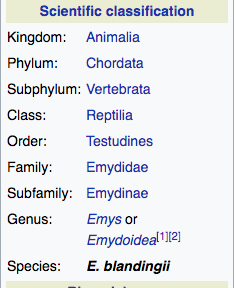
\includegraphics[scale=0.5]{testudines/emydidae/emydoidea/tax} \end{center}
	 \\
	\hline
	Size & 
	18-23 cm shell.
	\\
	\hline
	Color &
	bright yellow chin and throat. carapace specked w/ yellow/light-colored flecks/streaks on dark background. plastron yellow w/ symmetric dark blotches. dark head w/ yellow speckled legs. 
	 \\
	\hline
	Anatomy &
	the carapace is domed but slightly flattened along the midline, and oblong when viewed from above. it is also known as the ``semi-box" turtle b/c it has a hinged plastron, but the lobes do not shut as tightly as the box turtle. it may live to 80 years. since it does not demonstrate notable symptoms of aging until the end of its lifespan, it is considered senescent*.
	 \\
	\hline
	Dimorphism & 
	
	\\
	\hline
	Behavior & 
	very timid, it may plunge into the water and remain at the bottom for hours, or withdraw into the shell, when alarmed. very gentle, it rarely bites, and is an agile, good swimmer. it overwinters under or near water, in mud, or under vegetation or debris.
	\\
	\hline
	Habitat & 
	it inhabits wetlands w/ clean, shallow water. it can wander far from the water, especially for nesting or in search of a mating site or new food source.
	\\
	\hline
	Distribution & 
	range center = Great Lakes, extends from central Nebraska and Minnesota eastward through southern Ontario as far as northern NY. isolated populations in SE NY, New England, Nova Scotia.
	
	\begin{center} 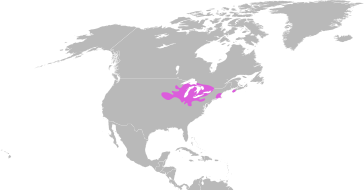
\includegraphics[scale=0.5]{testudines/emydidae/emydoidea/range} \end{center}
	\\
	\hline
	Feeding Ecology & 
	omnivorous, it consumes crustaceans and other invertebrates, fish, frogs, crayfish, carrion, berries, and vegetable debris. it is also capable of catching live fish.
	\\
	\hline
	Reproductive Biology & 
	it requires 14-20 years to reach sexual maturity. nesting takes place in early April-May, and nesting happens in early June. clutch size varies regionally; in New York, it is 5-12 eggs. females may be found more than a kilometer from where they hibernated during the mating season.
	\\
	\hline
	Ecological Role &
	
	\\
	\hline
	Conservation Status & 
	EN. primary threat = habitat fragmentation and nest predation by unnaturally large predator population. endangered in Indiana, Illinois, Missouri, Maine, New Hampshire, Massachusetts, and South Dakota.
	\\
	\hline
\end{longtabu}
\end{center}